\documentclass[10pt,a4paper]{report}
\usepackage[utf8]{inputenc}
% \usepackage[T1]{fontenc}
\usepackage{amsmath}
\usepackage{amsfonts}
\usepackage{amssymb}
\usepackage{graphicx}
\usepackage{textcomp}
\begin{document}

\begin{center}
\begin{Large}
Basic Linux Commands
\end{Large}
\end{center}
Experiment No.: 1\\
Date: 05/02/2019\\
Aim: Familiarization with basic Linux commands.\\
\\
Command 1: man\\
Purpose of Command: Display the manual page of the given command.\\
Usage: man [COMMAND]\\
Sample Input and Output: \\	
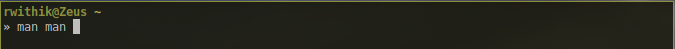
\includegraphics[scale=2]{man1.png}\\
\\
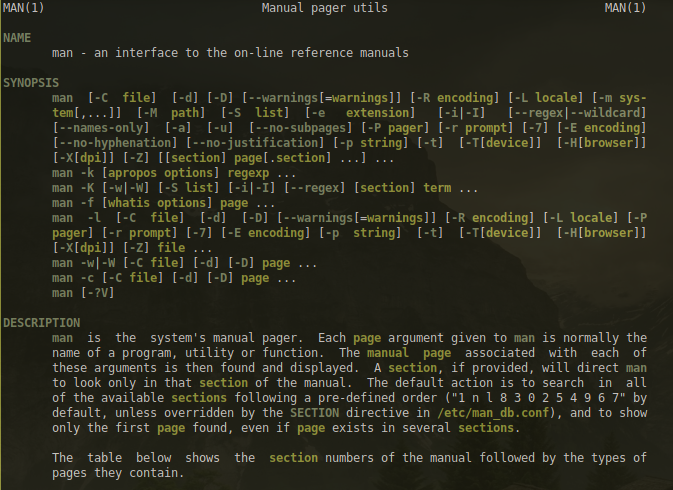
\includegraphics[scale=2]{man2.png}\\
\\
Command 2: ls\\
Purpose of Command: List the contents of the specified directory(The current directory, if no arguments are given.) Use -a flag to display all files, including hidden files. Use -l flag to display detailed information.\\
Usage: ls [PATH]\\
Sample Input and Output: \\
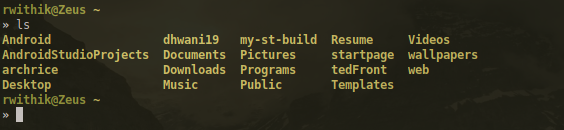
\includegraphics[scale=2]{ls.png}\\
\pagebreak
\\
Command 3: cd\\
Purpose of Command: Switch to the specified directory(Switches to the home directory, if no arguments are given.)\\
Usage: cd [PATH]\\
Sample Input and Output: \\
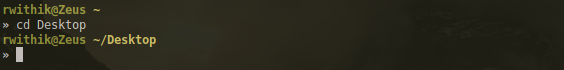
\includegraphics[scale=2]{cd.png}\\
\\
Command 4: pwd\\
Purpose of Command: Prints the present working directory.\\
Usage: pwd\\
Sample Input and Output: \\
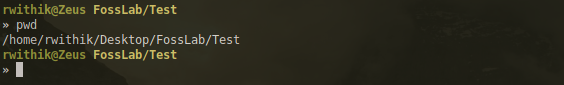
\includegraphics[scale=2]{pwd.png}\\
\\
Command 5: echo\\
Purpose of Command: Print to the terminal.\\
Usage: echo [ARGS]\\
Sample Input and Output: \\
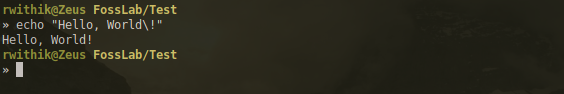
\includegraphics[scale=2]{echo.png}\\
\\
Command 6: mkdir\\
Purpose of Command: Creates a directory with the given name. Use the -p flag to automatically create athe requiured parent directories.\\
Usage: cd [NAME]\\
Sample Input and Output: \\
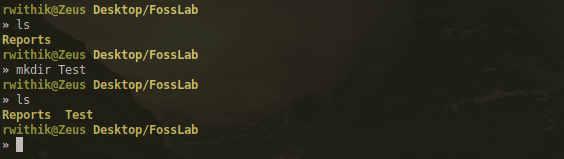
\includegraphics[scale=2]{mkdir.png}\\
\pagebreak
\\
Command 7: touch\\
Purpose of Command: Creates a file with the given name.\\
Usage: touch [FILENAME]\\
Sample Input and Output: \\
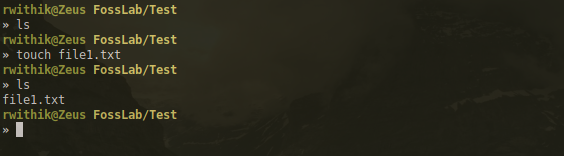
\includegraphics[scale=2]{touch.png}\\
\\
Command 8: cp\\
Purpose of Command: Copy files and directories from one location to another. Use the -r flag to copy directories.\\
Usage: cp [SOURCE] [DESTINATION]\\
Sample Input and Output: \\
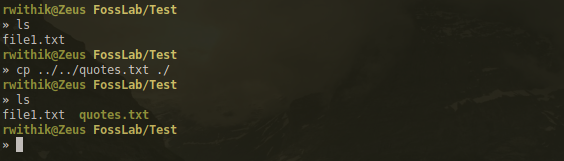
\includegraphics[scale=2]{cp.png}\\
\\
Command 9: mv\\
Purpose of Command: Move files and directories.\\
Usage: mv [SOURCE] [DESTINATION]\\
Sample Input and Output: \\
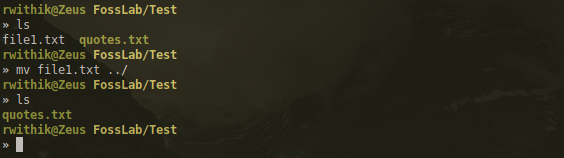
\includegraphics[scale=2]{mv.png}\\
\pagebreak
\\
Command 10: rm\\
Purpose of Command: Delete files and directories. Use the -r flag to delete directories.\\
Usage: rm [PATH]\\
Sample Input and Output: \\
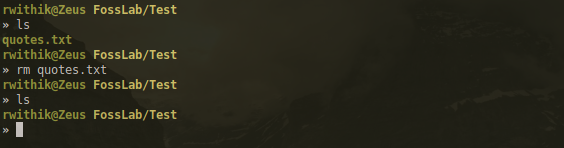
\includegraphics[scale=2]{rm.png}\\
\\
Command 11: tree\\
Purpose of Command: Displays the contents of a folder in tree structure.\\
Usage: tree [PATH]\\
Sample Input and Output: \\
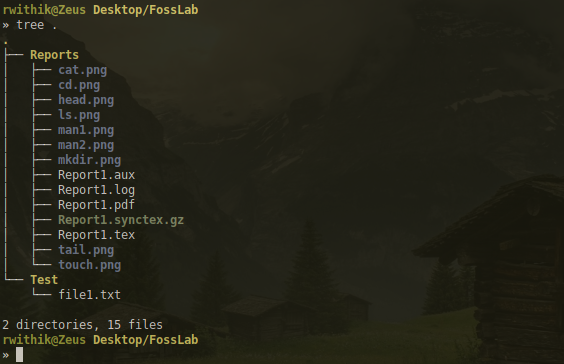
\includegraphics[scale=.5]{tree.png}\\
\pagebreak
\\
Command 12: cat\\
Purpose of Command: Prints the contents of the given files. Use the -n flag to display line numbers.\\
Usage: cat [FILE1] [FILE2] [FILE3] ...\\
Sample Input and Output: \\
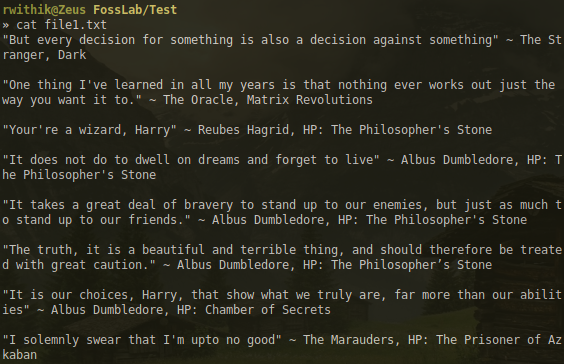
\includegraphics[scale=.5]{cat.png}\\
\\
Command 13: head\\
Purpose of Command: Prints the first few lines(10, by default) of the given file. Use the -n flag to display more(or less) lines.\\
Usage: head [FILE]\\
Sample Input and Output: \\
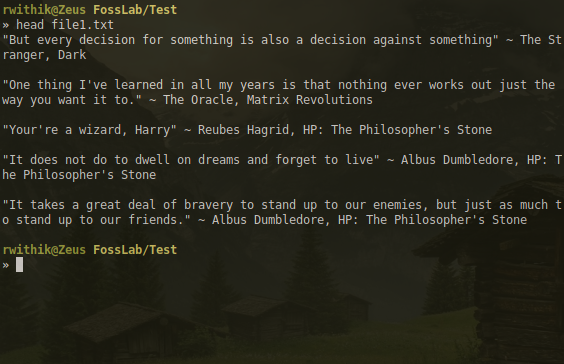
\includegraphics[scale=.5]{head.png}\\
\pagebreak
\\
Command 14: tail\\
Purpose of Command: Prints the last few lines(10, by default) of the given file. Use the -n flag to display more(or less) lines.\\
Usage: tail [FILE]\\
Sample Input and Output: \\
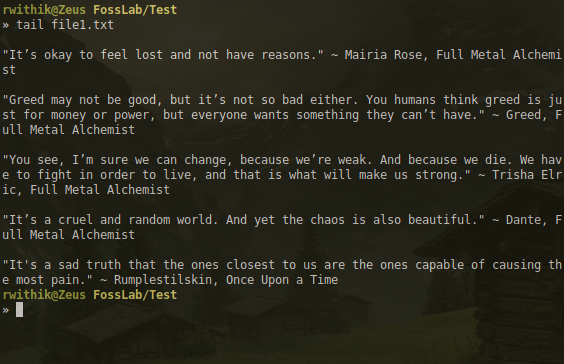
\includegraphics[scale=.5]{tail.png}\\
\\
Command 15: less\\
Purpose of Command: Prints the contents of a file, one screen at a time.\\
Usage: less [FILE]\\
Sample Input and Output: \\
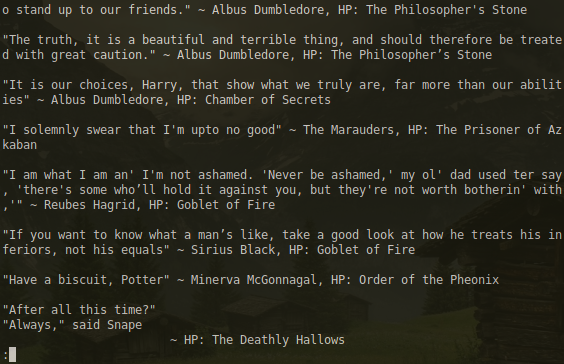
\includegraphics[scale=.5]{less.png}\\
\pagebreak
\\
Command 16: chmod\\
Purpose of Command: Change the permissions of a file or directory.\\
Usage: chmod [PERMISSIONS] [PATH]\\
Sample Input and Output: \\
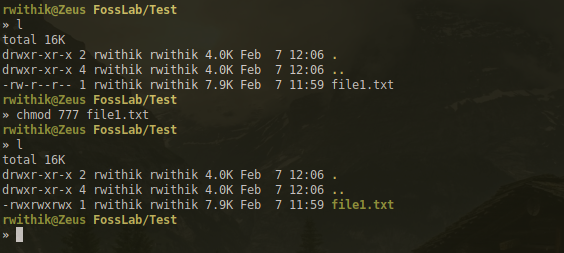
\includegraphics[scale=2]{chmod.png}\\
\\

\pagebreak

\begin{center}
\begin{Large}
Linux Commands for Operations
\end{Large}
\end{center}
Experiment No.: 2\\
Date: 05/02/2019\\
Aim: Familiarization with Linux Commands for Operations.\\
\\
Operation 1: Redirection\\
Purpose: Redirect the output of one command to another file, or stream.\\
Usage: [COMMAND1] $>$ [COMMAND2]\\
{[COMMAND1]} $>>$ [COMMAND2]\\
Sample Input and Output:\\
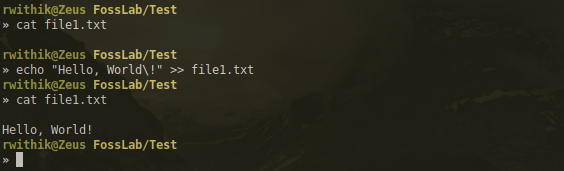
\includegraphics[scale=2]{redirection.png}\\
\\
Operation 2: Piping\\
Purpose: Give the output of one command to another command.\\
Usage: [COMMAND1] $|$ [COMMAND2]\\
Sample Input and Output:\\
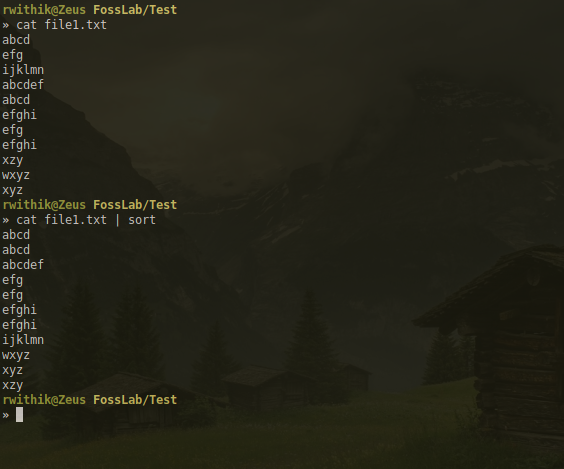
\includegraphics[scale=.5]{piping.png}\\
\pagebreak
\\
Operation 3: sort\\
Purpose: Sort the output. Use the -r flag to sort it in reverse order.\\
Usage: [COMMAND] $|$ sort\\
Sample Input and Output:\\
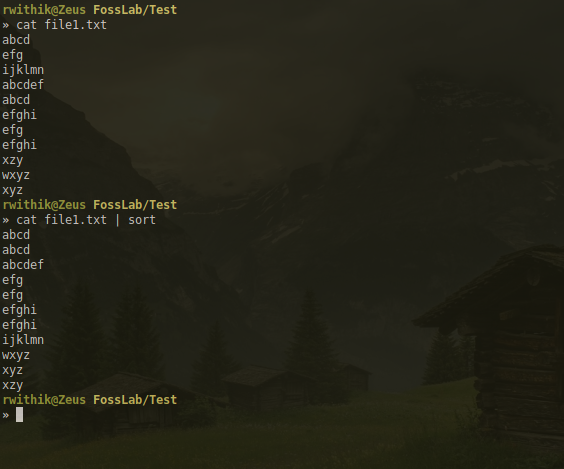
\includegraphics[scale=.5]{sort.png}\\
\\
Operation 4: uniq\\
Purpose: Excludes adjacent identical lines from the input.\\
Usage: [COMMAND1] $|$ uniq\\
Sample Input and Output:\\
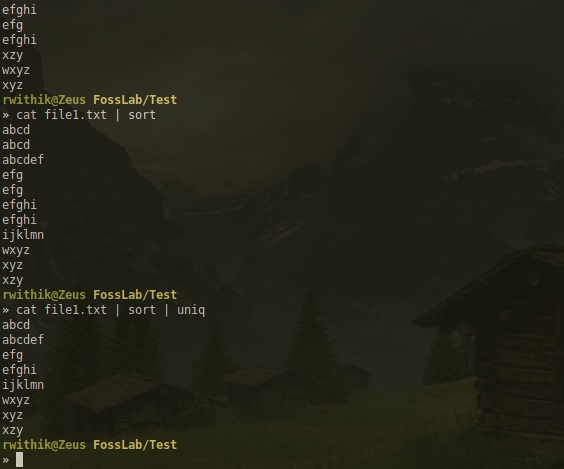
\includegraphics[scale=.5]{uniq.png}\\
\pagebreak
\\
Operation 5: Job Control- Display\\
Purpose: Display the jobs in the background\\
Usage: jobs\\
Sample Input and Output:\\
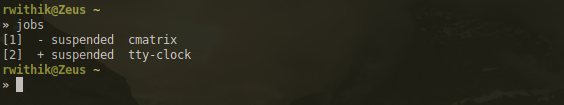
\includegraphics[scale=2]{jobdisplay.png}\\
\\
Operation 6: Job Control- Kill\\
Purpose: Kill the specifies job.\\
Usage: kill [PID]\\
killall [NAME]\\
Sample Input and Output:\\

\includegraphics[scale=2]{kill.png}\\
\\
Operation 7: ps\\
Purpose: Display the active processes in the current shell session.\\
Usage: ps\\
Sample Input and Output:\\
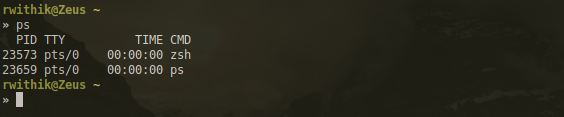
\includegraphics[scale=2]{ps.png}\\
\\


\pagebreak

\begin{center}
\begin{Large}
Advanced Linux Commands
\end{Large}
\end{center}
Experiment No.: 3\\
Date: 05/02/2019\\
Aim: Familiarization with Advanced Linux Commands.\\
\\
Command 1: curl\\
Purpose: Send and receive data from and to a server.\\
Usage: curl [URLs]\\
Sample Input and Output: \\
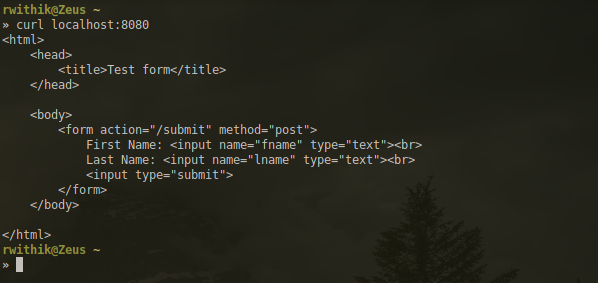
\includegraphics[scale=2]{curl.png}\\
\\
Command 2: wget\\
Purpose: \\
Usage: wget [URLs]\\
Sample Input and Output: \\
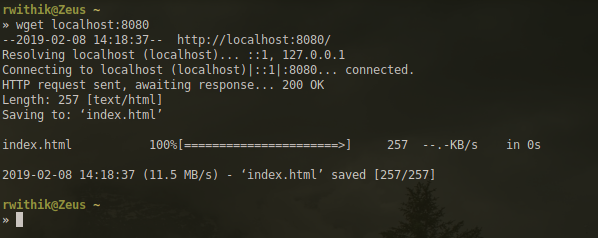
\includegraphics[scale=2]{wget.png}\\
\\
Command 3: ftp\\
Purpose: Remote file transfer with File Transfer Protocol.\\
Usage: ftp [IP or DOMAIN]\\
Sample Input and Output: \\
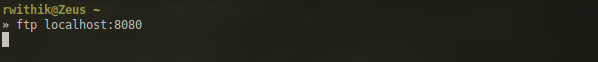
\includegraphics[scale=2]{ftp.png}\\
\pagebreak
\\
Command 4: ssh\\
Purpose: Program for logging into a remote machine and for executing commands on it over a network.\\
Usage: ssh [username@domain]\\
Sample Input and Output: \\
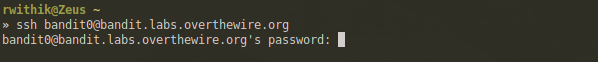
\includegraphics[scale=2]{ssh.png}\\
\\
Command 5: grep\\
Purpose: Searches for the given pattern in the given files. Use the -e flag for regex support.\\
Usage: grep [PATTERN] [FILE]\\
{[COMMAND]} $|$ grep [PATTERN]\\
Sample Input and Output: \\
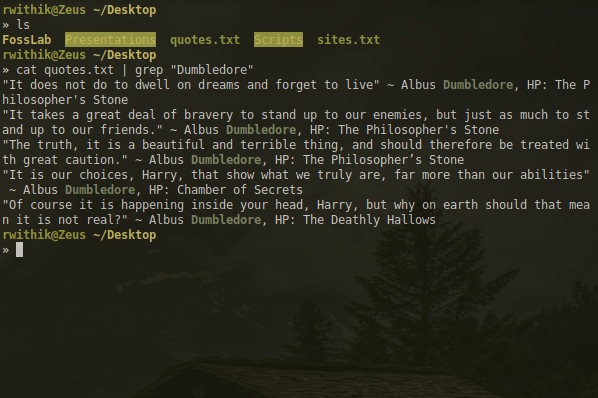
\includegraphics[scale=.5]{grep.png}

\end{document}